% vim: set tw=0:
\documentclass{beamer}
\usepackage{graphicx}
\usepackage{hyperref}
\hypersetup{pdfborder={0 0 0 0}}

% Reasonable themes:
% Antibes Bergen Berkeley Berlin Frankfurt Goettingen Ilmenau Luebeck Malmoe
% Montpellier PaloAlto Rochester Singapore Szeged Warsaw bars boxes
% compatibility default lined plain shadow sidebar split tree
% And these ones include the author's name on every slide:
% Berkeley

% Declare themes.
\mode<presentation>
\usetheme{UWHEP}

% Personal macros.
\newcommand{\email}[1]{{\texttt #1}}
\newcommand{\newframe}[1]{\section{#1}
    \frametitle{\sc{#1}}}
\newcommand{\subframe}[1]{\subsection{#1}
    \frametitle{\sc{#1}}}
\newcommand{\supers}[1]{\ensuremath{^\textrm{#1}}}
\newcommand{\subs}[1]{\ensuremath{_\textrm{#1}}}
\newcommand{\ca}{\ensuremath{\sim}}
\renewcommand{\email}[1]{\href{mailto:#1}{\nolinkurl{#1}}}

% Author information.
\title{T2 Status}
\author[Maier, Mohapatra]{
    Will Maier \and Ajit Mohapatra\\ 
    {\tt wcmaier@hep.wisc.edu}\\
    {\tt ajit@hep.wisc.edu}}
\institute[Wisconsin]{University of Wisconsin - High Energy Physics}
\date{2009.05.26}
\logo{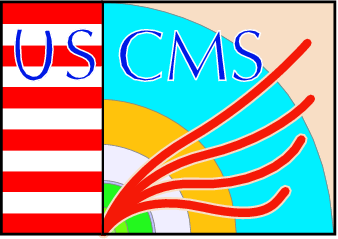
\includegraphics[height=0.6cm]{../../../Graphics/USCMS_logo.png}\hspace{.1cm}
\includegraphics[height=0.75cm]{../../../Graphics/UW_logo.png}}

\begin{document}

\begin{frame}
    \titlepage
\end{frame}

%\section{Overview}
%\begin{frame}
%    \tableofcontents
%\end{frame}

\section{Facilities}
\subsection{Software and Storage}
\begin{frame}
\frametitle{}
\begin{itemize}
	\item Built and benchmarked new RAID for PNFS server and MC DB host
	\begin{itemize}
		\item 4-5x performance improvement in disk IO over current hardware
		\item Should decrease cost of namespace lookups
	\end{itemize}
	\item CRAB user submitted jobs against dataset that hasn't been finished
	\begin{itemize}
		\item Files still staging to FNAL (and getting cleaned up locally by PhEDEx)
		\item Should (or does?) CRAB prevent this?
	\end{itemize}
	\item Jobs on Nehalem test system for opportunistic resources upgrade showed 8\% improvement over similar hardware
	\item Redownloaded corrupt file discovered by Ken
	\item Wrote and deployed a lightweight dCache replicator
	\begin{itemize}
		\item Follows billing log and issues replications for each new file
		\item Low-latency first approximation of replication policy
		\item PFM is slower but more accurate -- they work well together
		\item {\tt easy\_install dcache-tools}; \url{http://code.hep.wisc.edu/dcache-tools}
	\end{itemize}
\end{itemize}
\end{frame}

\subsection{Production and Monitoring}
\begin{frame}
\frametitle{}
\begin{itemize}
     \item JobRobot: OK
     \item SAM: Some SRM timeouts due to load
     \item RSV: OK
     \item PhEDEx:
	 \begin{itemize}
		\item Intermittent xfer errors in LT due to SRM overload (grid-ftp-copy timeout; see SAM above) 
		\item Cleaning up full dcache
		\item Usual MC xfers from local users
	 \end{itemize}
     \item MC Production:
	 \begin{itemize}
		\item We are getting close on the Summer08 production (finally)
		\item Last bits of Alpgen and a couple of DPG cosmics finishing
		\item 3\_1\_X production planning is continuing
	 \end{itemize}
\end{itemize}
\end{frame}

\end{document}
